\documentclass{article}\usepackage[]{graphicx}\usepackage[]{color}
% maxwidth is the original width if it is less than linewidth
% otherwise use linewidth (to make sure the graphics do not exceed the margin)
\makeatletter
\def\maxwidth{ %
  \ifdim\Gin@nat@width>\linewidth
    \linewidth
  \else
    \Gin@nat@width
  \fi
}
\makeatother

\definecolor{fgcolor}{rgb}{0.345, 0.345, 0.345}
\makeatletter
\@ifundefined{AddToHook}{}{\AddToHook{package/xcolor/after}{\definecolor{fgcolor}{rgb}{0.345, 0.345, 0.345}}}
\makeatother
\newcommand{\hlnum}[1]{\textcolor[rgb]{0.686,0.059,0.569}{#1}}%
\newcommand{\hlstr}[1]{\textcolor[rgb]{0.192,0.494,0.8}{#1}}%
\newcommand{\hlcom}[1]{\textcolor[rgb]{0.678,0.584,0.686}{\textit{#1}}}%
\newcommand{\hlopt}[1]{\textcolor[rgb]{0,0,0}{#1}}%
\newcommand{\hlstd}[1]{\textcolor[rgb]{0.345,0.345,0.345}{#1}}%
\newcommand{\hlkwa}[1]{\textcolor[rgb]{0.161,0.373,0.58}{\textbf{#1}}}%
\newcommand{\hlkwb}[1]{\textcolor[rgb]{0.69,0.353,0.396}{#1}}%
\newcommand{\hlkwc}[1]{\textcolor[rgb]{0.333,0.667,0.333}{#1}}%
\newcommand{\hlkwd}[1]{\textcolor[rgb]{0.737,0.353,0.396}{\textbf{#1}}}%
\let\hlipl\hlkwb

\usepackage{framed}
\makeatletter
\newenvironment{kframe}{%
 \def\at@end@of@kframe{}%
 \ifinner\ifhmode%
  \def\at@end@of@kframe{\end{minipage}}%
  \begin{minipage}{\columnwidth}%
 \fi\fi%
 \def\FrameCommand##1{\hskip\@totalleftmargin \hskip-\fboxsep
 \colorbox{shadecolor}{##1}\hskip-\fboxsep
     % There is no \\@totalrightmargin, so:
     \hskip-\linewidth \hskip-\@totalleftmargin \hskip\columnwidth}%
 \MakeFramed {\advance\hsize-\width
   \@totalleftmargin\z@ \linewidth\hsize
   \@setminipage}}%
 {\par\unskip\endMakeFramed%
 \at@end@of@kframe}
\makeatother

\definecolor{shadecolor}{rgb}{.97, .97, .97}
\definecolor{messagecolor}{rgb}{0, 0, 0}
\definecolor{warningcolor}{rgb}{1, 0, 1}
\definecolor{errorcolor}{rgb}{1, 0, 0}
\makeatletter
\@ifundefined{AddToHook}{}{\AddToHook{package/xcolor/after}{
\definecolor{shadecolor}{rgb}{.97, .97, .97}
\definecolor{messagecolor}{rgb}{0, 0, 0}
\definecolor{warningcolor}{rgb}{1, 0, 1}
\definecolor{errorcolor}{rgb}{1, 0, 0}
}}
\makeatother
\newenvironment{knitrout}{}{} % an empty environment to be redefined in TeX

\usepackage{alltt}

\usepackage[sc]{mathpazo}
\usepackage[T1]{fontenc}
\usepackage[left=1in,top=1in,right=1in,bottom=1in,headheight=3ex,headsep=3ex]{geometry}
\usepackage{graphicx}
\usepackage{float}
\usepackage{xcolor}
\usepackage{tikz}
\usetikzlibrary{tikzmark}
\usetikzlibrary{matrix}
\tikzset{ 
table/.style={
  matrix of nodes,
  row sep=-\pgflinewidth,
  column sep=-\pgflinewidth,
  nodes={rectangle,text width=3em,align=center},
  text depth=1.25ex,
  text height=2.5ex,
  nodes in empty cells
},
%row 1/.style={nodes={fill=green!10,text depth=0.4ex,text height=2ex}},
%row 6/.style={nodes={text depth=0.4ex,text height=2ex}},
%column 1/.style={nodes={fill=green!10}},
}
\usepackage{amsmath}
\DeclareMathOperator*{\argmax}{\arg\!\max} 
\newcommand{\blankline}{\quad\pagebreak[2]}
\geometry{verbose,tmargin=2.5cm,bmargin=2.5cm,lmargin=2.5cm,rmargin=2.5cm}
\setcounter{secnumdepth}{2}
\setcounter{tocdepth}{2}
\usepackage{hyperref}
\hypersetup{
    colorlinks=true,
    linkcolor=blue,
    filecolor=magenta,      
    urlcolor=blue,
    pdfpagemode=FullScreen,
    }
    \setlength{\parindent}{0pt}
\IfFileExists{upquote.sty}{\usepackage{upquote}}{}
\begin{document}



\title{COMP 5970/6970-004 \\ Computational Biology: Genomics and Transcriptomics \\ Homework 1 solutions }
\author{Haynes Heaton}
\date{Spring, 2022}


\maketitle
\blankline

\begin{tabular*}{.93\textwidth}{@{\extracolsep{\fill}}lr}

%%%%%%%%%%%%%%%%%%%%%%%%%%%%%%%%%%%%%%%%%%%%%%%%%%%%%%%%%%%%%%

% Modify information %%%%%%%%%%%%%%%%%%%%%%%%%%%%%%%%%%%%%%%%%

\hline
\end{tabular*}


\textbf{Question 2:} What is the property that makes problems amenable to solutions using dynamic programming? \\ \\
Answer: Given a base case solution and a solution at point $i$, there is an easy way to find the optimal solution at point $i+1$. This is the inductive property. Partial credit given to any answer about combining sub problems as that is also applicable to divide and conquer. \\ \\

\textbf{Question 3:} True or False, in global alignment with scoring system match: +1, mismatch: -1, indel: -1, the score can go up when coming from a horizontal or vertical prior cell in the scoring matrix. \\ \\
Answer: False, all moves vertical or horizontal are indels and thus reduce the alignment score. \\ \\

\textbf{Question 4:} What is the formal name of the backtrace algorithm? \\ \\
Answer: Viterbi algorithm \\ \\

\textbf{Question 5:} Provide two different optimal solutions for the global alignment of GCAGTC and GACTGC in the form of two lines of strings with dashes for indels. Switching to courier new font will make it look nicer (monospaced fonts will make the two lines match character for character) \\ \\
Answer: \\ 

\noindent
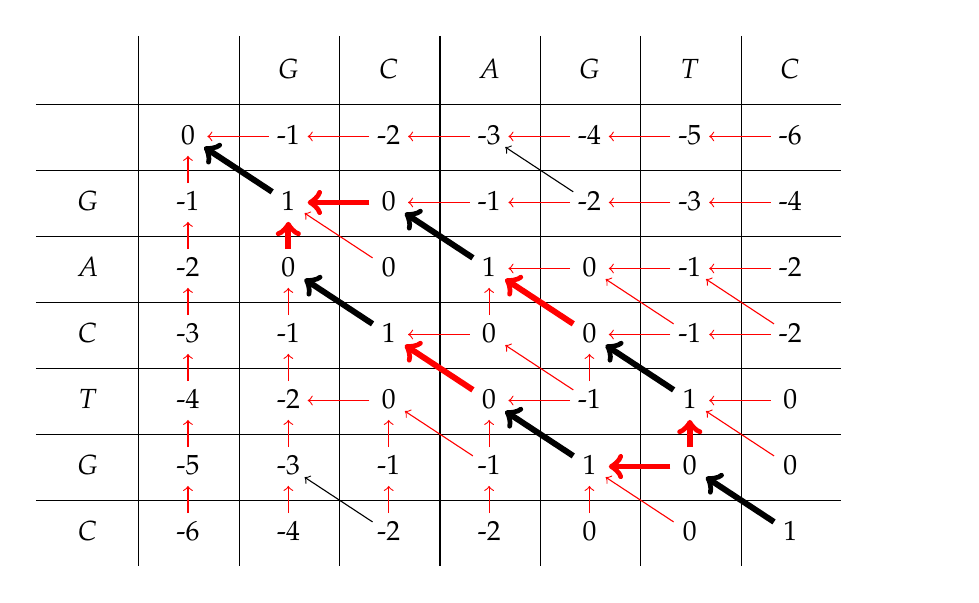
\begin{tikzpicture}[scale=0.8]
\matrix (mat) [table]
{
& & $G$ & $C$ & $A$ & $G$ & $T$ & $C$  \\
&0  & -1 &-2 & -3 & -4 & -5 & -6 &  \\
$G$ & -1 & 1 & 0 & -1 & -2 & -3 & -4 \\
$A$ & -2 & 0 & 0 & 1 & 0 & -1 & -2 \\
$C$ & -3 & -1 & 1 & 0 & 0 & -1 & -2\\
$T$ & -4 & -2 & 0 & 0 & -1 &1  &0\\
$G$ & -5 & -3&-1 &-1 &1 &0 & 0\\
$C$ & -6 &-4 &-2 &-2 &0 &0 &1 \\
};
% the matrix rules
\foreach \x in {1,...,7}
{
  \draw 
    ([xshift=-.5\pgflinewidth]mat-\x-1.south west) --   
    ([xshift=-.5\pgflinewidth]mat-\x-8.south east);
  }
\foreach \x in {1,...,7}
{
  \draw 
    ([yshift=.5\pgflinewidth]mat-1-\x.north east) -- 
    ([yshift=.5\pgflinewidth]mat-8-\x.south east);
}    
% the arrows
\begin{scope}[shorten >=7pt,shorten <= 7pt]
\draw[line width =.75mm,->]  (mat-3-3.center) -- (mat-2-2.center);
\draw[red,->]  (mat-2-3.center) -- (mat-2-2.center);
\draw[red,->]  (mat-2-4.center) -- (mat-2-3.center);
\draw[red,->]  (mat-2-5.center) -- (mat-2-4.center);
\draw[red,->]  (mat-2-6.center) -- (mat-2-5.center);
\draw[red,->]  (mat-2-7.center) -- (mat-2-6.center);
\draw[red,->]  (mat-2-8.center) -- (mat-2-7.center);
\draw[red,->]  (mat-3-2.center) -- (mat-2-2.center);
\draw[red,->]  (mat-4-2.center) -- (mat-3-2.center);
\draw[red,->]  (mat-5-2.center) -- (mat-4-2.center);
\draw[red,->]  (mat-6-2.center) -- (mat-5-2.center);
\draw[red,->]  (mat-7-2.center) -- (mat-6-2.center);
\draw[red,->]  (mat-8-2.center) -- (mat-7-2.center);
\draw[line width =.75mm,red,->]  (mat-3-4.center) -- (mat-3-3.center);
\draw[red,->]  (mat-3-5.center) -- (mat-3-4.center);
\draw[->]  (mat-3-6.center) -- (mat-2-5.center);
\draw[red,->]  (mat-3-6.center) -- (mat-3-5.center);
\draw[red,->]  (mat-3-7.center) -- (mat-3-6.center);
\draw[red,->]  (mat-3-8.center) -- (mat-3-7.center);
\draw[line width =.75mm,red,->]  (mat-4-3.center) -- (mat-3-3.center);
\draw[red,->]  (mat-4-4.center) -- (mat-3-3.center);
\draw[line width =.75mm,->]  (mat-4-5.center) -- (mat-3-4.center);
\draw[red,->]  (mat-4-6.center) -- (mat-4-5.center);
\draw[red,->]  (mat-4-7.center) -- (mat-4-6.center);
\draw[red,->]  (mat-4-8.center) -- (mat-4-7.center);
\draw[red,->]  (mat-5-3.center) -- (mat-4-3.center);
\draw[line width =.75mm,->]  (mat-5-4.center) -- (mat-4-3.center);
\draw[red,->]  (mat-5-5.center) -- (mat-5-4.center);
\draw[red,->]  (mat-5-5.center) -- (mat-4-5.center);
\draw[line width =.75mm,red,->]  (mat-5-6.center) -- (mat-4-5.center);
\draw[red,->]  (mat-5-7.center) -- (mat-4-6.center);
\draw[red,->]  (mat-5-7.center) -- (mat-5-6.center);
\draw[red,->]  (mat-5-8.center) -- (mat-5-7.center);
\draw[red,->]  (mat-5-8.center) -- (mat-4-7.center);
\draw[red,->]  (mat-6-3.center) -- (mat-5-3.center);
\draw[red,->]  (mat-6-4.center) -- (mat-6-3.center);
\draw[line width =.75mm,red,->]  (mat-6-5.center) -- (mat-5-4.center);
\draw[red,->]  (mat-6-6.center) -- (mat-5-5.center);
\draw[red,->]  (mat-6-6.center) -- (mat-6-5.center);
\draw[red,->]  (mat-6-6.center) -- (mat-5-6.center);
\draw[line width =.75mm,->]  (mat-6-7.center) -- (mat-5-6.center);
\draw[red,->]  (mat-6-8.center) -- (mat-6-7.center);
\draw[red,->]  (mat-7-3.center) -- (mat-6-3.center);
\draw[red,->]  (mat-7-4.center) -- (mat-6-4.center);
\draw[red,->]  (mat-7-5.center) -- (mat-6-4.center);
\draw[red,->]  (mat-7-5.center) -- (mat-6-5.center);
\draw[line width =.75mm,->]  (mat-7-6.center) -- (mat-6-5.center);
\draw[line width =.75mm,red,->]  (mat-7-7.center) -- (mat-6-7.center);
\draw[line width =.75mm,red,->]  (mat-7-7.center) -- (mat-7-6.center);
\draw[red,->]  (mat-7-8.center) -- (mat-6-7.center);
\draw[red,->]  (mat-8-3.center) -- (mat-7-3.center);
\draw[->]  (mat-8-4.center) -- (mat-7-3.center);
\draw[red,->]  (mat-8-4.center) -- (mat-7-4.center);
\draw[red,->]  (mat-8-5.center) -- (mat-7-5.center);
\draw[red,->]  (mat-8-6.center) -- (mat-7-6.center);
\draw[red,->]  (mat-8-7.center) -- (mat-7-6.center);
\draw[line width =.75mm,->]  (mat-8-8.center) -- (mat-7-7.center);
\end{scope}
\end{tikzpicture} \\

Giving us two optimal alignments of \\
(upper path) \\
\texttt{GCAGT-C} \\
\texttt{G-ACTGC} \\ 
(and lower path) \\
\texttt{G-CAGTC} \\
\texttt{GACTG-C} \\ \\

\textbf{Question 6:}  What is the final score (number in lower right cell in the scoring matrix) of question 5? \\ \\
Answer: 1 \\ \\

\textbf{Question 7:} Describe a dynamic programming approach to finding the largest checkerboard pattern in a matrix of zeros and ones where zero represents white and one represents black (checkerboard pattern is just alternating 0s and 1s, it does not matter which color starts or ends the pattern). Checkerboard must be square. Don't spend over an hour on this. If you find it difficult, come to my office hours after class and we can work through it together. Starting with 7a may help. And coming up with rules and testing them out may lead to the correct rules so use the example matrix below. \\ \\
Answer: 
\noindent
Generally in dynamic programming you will have a table that keeps track of the optimal solution(s) up to this point. We need to decide what our base case solution is. In this case, the simplest base cases to use would be a $0x0$ size checkerboard or a $1x1$ checkerboard. For this example, I will use $1x1$. So a single cell of $1$ or $0$ are both $1x1$ checkerboards. Now we need to decide what the values in the DP table represent. Similar to our global alignment problem, we could have a DP table of the same size as the input matrix. In the global alignment problem, the value was the score of the alignment up until now. Here it is natural to make the DP table keep track of the largest checkerboard cell $i,j$ is the bottom right corner of. If that is the case, the left column and top row are all the base case of a $1x1$ checkerboard. We will denote the input matrix $I$ and the DP table $S$ for score. So the DP table $S$ is initialized as
\noindent
\begin{tikzpicture}
\matrix (mat) [table]
{
& & & &  &  &  & \\
& 1&1&1&1&1&1& \\
 & 1& & & & & &\\
 & 1& &  & & & &\\
 & 1& & & &  & &\\
 & 1& & & & &  &\\
 & & & & & & & \\
};
% the matrix rules
\foreach \x in {1,...,6}
{
  \draw 
    ([xshift=0\pgflinewidth]mat-\x-2.south west) --   
    ([xshift=0\pgflinewidth]mat-\x-7.south east);
  }
\foreach \x in {1,...,7}
{
  \draw 
    ([yshift=1\pgflinewidth]mat-2-\x.north east) -- 
    ([yshift=1\pgflinewidth]mat-6-\x.south east);
}    
% the arrows
\end{tikzpicture}

\noindent
Now at each $i=1..n$ and $j=1..m$, we can check the cell above and to the left of it in the input matrix and make sure they are different and the one diagonal to the upper left and make sure they are they same. If that is the case, this square is the bottom right of a checkerboard that is $min(S[i-1][j-1], S[i][j-1], S[i-1][j]) + 1$. If this isn't the case, this is only the base case checkerboard of $1x1$. So our formal recurrence relation is
\begin{equation*}
S[i,j] = 
\begin{cases}
      min(S[i-1,j-1], S[i-1][j], S[i][j-1]) + 1\\ 
      \text{\,\,\,\,\,\,\,\,\,\,\,\,if\,\,} I[i][j] = I[i-1][j-1]  \\
      \text{\,\,\,\,\,\,\,\,\,\,\,\,\,\,\,\,\,\,\,and\,\,} I[i][j] \neq I[i-1][j] \\
      \text{\,\,\,\,\,\,\,\,\,\,\,\,\,\,\,\,\,\,\,and\,\,} I[i][j] \neq I[i][j-1] \text{\,\,\,(continuation of a checkerboard)} \\
      1 \text{\,\,\,otherwise} \\
\end{cases}
\end{equation*}
So filling the DP table out, we have 

\noindent
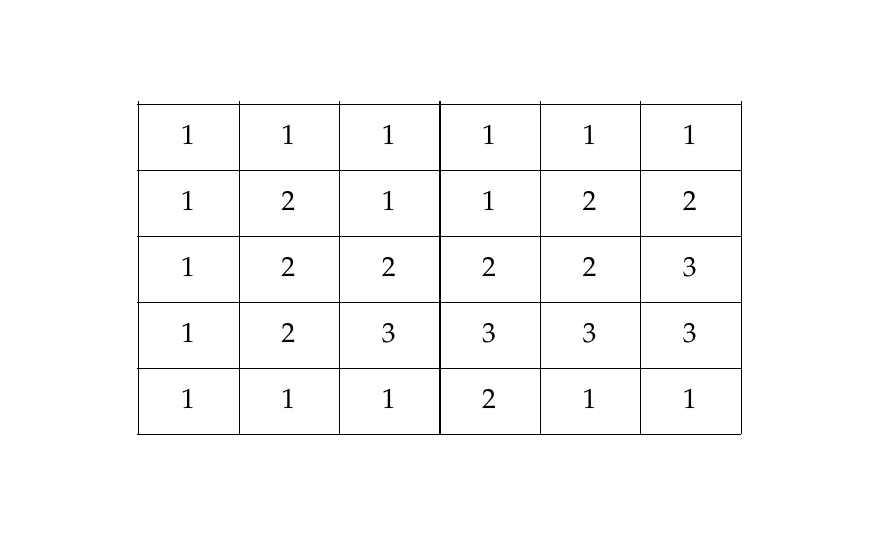
\begin{tikzpicture}
\matrix (mat) [table]
{
& & & &  &  &  & \\
& 1&1&1&1&1&1& \\
 & 1&2 & 1& 1& 2&2 &\\
 & 1& 2& 2 & 2& 2& 3&\\
 & 1& 2&3 & 3&  3&3 &\\
 & 1&1 & 1& 2& 1& 1 &\\
 & & & & & & & \\
};
% the matrix rules
\foreach \x in {1,...,6}
{
  \draw 
    ([xshift=0\pgflinewidth]mat-\x-2.south west) --   
    ([xshift=0\pgflinewidth]mat-\x-7.south east);
  }
\foreach \x in {1,...,7}
{
  \draw 
    ([yshift=1\pgflinewidth]mat-2-\x.north east) -- 
    ([yshift=1\pgflinewidth]mat-6-\x.south east);
}    
% the arrows
\end{tikzpicture} \\
\noindent
So we have several ties for different locations of a $3x3$ checkerboard in the given input matrix. \\ \\

\textbf{Question 7a:}  What is the base case for this algorithm? \\ \\
Answer: 1x1 checkerboard of either 0 or 1. Also 0x0 would be acceptable. And since I didn't give a formal definition of a checkerboard, I also accepted 2x2. \\ \\

\end{document}
